\chapter{Ergebnisse} \label{chapter:ergebnisse}
\section{Generierung von $\beta_2$-Adrenorezeptoren mit dem SNAP-tag} \label{klonierung}
Zur Untersuchung der Oligomerisierung des \gls{beta2} wurde der Rezeptor so modifiziert, dass er über eine extrazelluläre Komponente verfügte, die Untersuchungen mit fluoreszierenden Substraten ermöglichte. Der SNAP-tag ermöglicht über seine O\textsuperscript{6}-Alkylguanin-DNA-Alkyltransferase-Aktivität die kovalente Bindung nahezu beliebiger Moleküle \parencite{Gronemeyer2006}. Die gewünschten Fluorophore müssen dazu eine O\textsuperscript{6}-Benzylguanin oder O\textsuperscript{6}-Alkylguanin-Gruppe tragen. Viele Fluorophore, darunter trFRET-kompatible, sind kommerziell verfügbar. Die Funktionsweise ist in Abbildung \ref{fig:snap-tag} dargestellt

\begin{figure}[htp]
    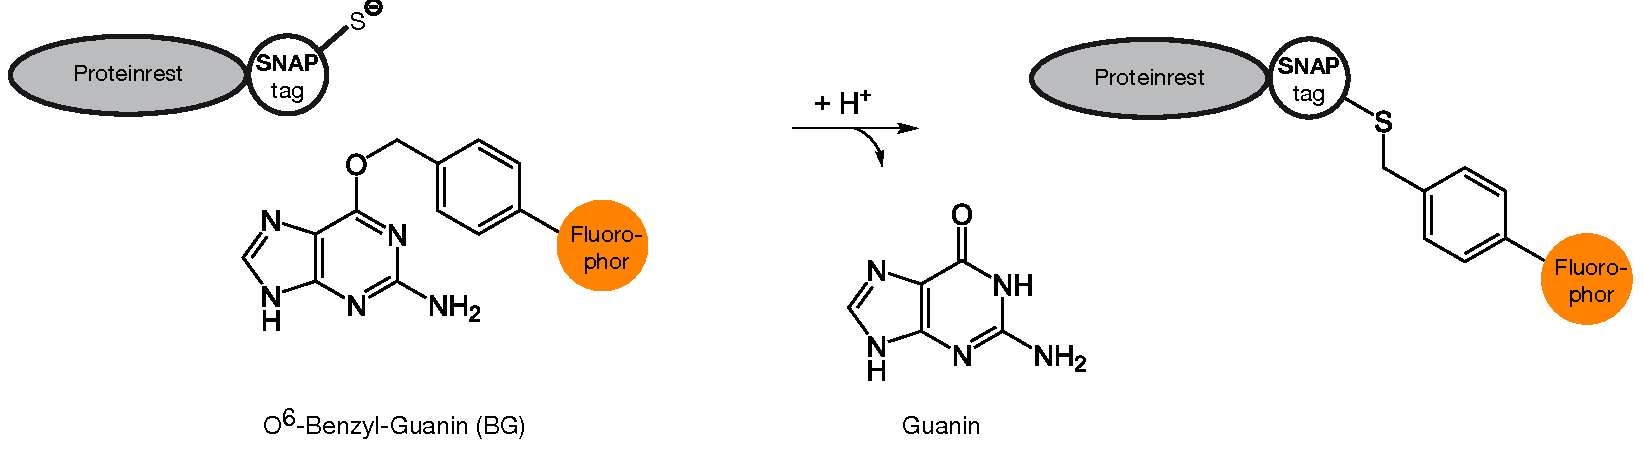
\includegraphics[width=0.97\textwidth]{SNAP-tag.pdf}
    \caption{\textbf{Funktionsweise des SNAP-tag}}
    \label{fig:snap-tag}
\end{figure}

Darauf basierend wurden Vektoren kloniert, die den \gls{beta2} trugen, der N-terminal über den SNAP-tag verfügte. 
\\ \\
Mittels Fluoreszenzmikroskopie konnte initial gezeigt werden, dass mit der N-terminalen Modifikation des \gls{beta2} keine Membranexpression des \gls{beta2} mehr erfolgte (s. Abb. \ref{fig:stainsnap} in \ref{snapmikro}). Infolgedessen wurde weiter N-terminal eine Proteinsequenz zur Membraninsertion verwendet, die zur zufriedenstellenden Expression des \gls{beta2} führte. 
\\ \\
In Abbildung \ref{fig:klonierung} sind schematisch die Klonierungsstrategien zu den final verwendeten Vektoren dargestellt. Es wurden Expressionsvektoren erzeugt, die die SNAP-getaggten natürlich vorkommenden Varianten Arg16 und Gly16 des \gls{beta2} exprimierten.
\\ \\ 
Darüber hinaus wurden zwei weitere Expressionssysteme generiert: Ein Vektor, der den \gls{beta2} mit dem SNAP-tag im zweiten extrazellulären Loop trug, sowie einen weiteren, der die in der Literatur als dimerisierungsdefizient beschriebene Variante Tyr284 \parencite{Salahpour2004} enthielt.
\\ \\
Für zukünftige Anwendung wurden außerdem analog Vektoren kloniert, die den mit dem CLIP-tag versehenen \gls{beta2} trugen (nicht dargestellt). 

\begin{figure}[htp]
    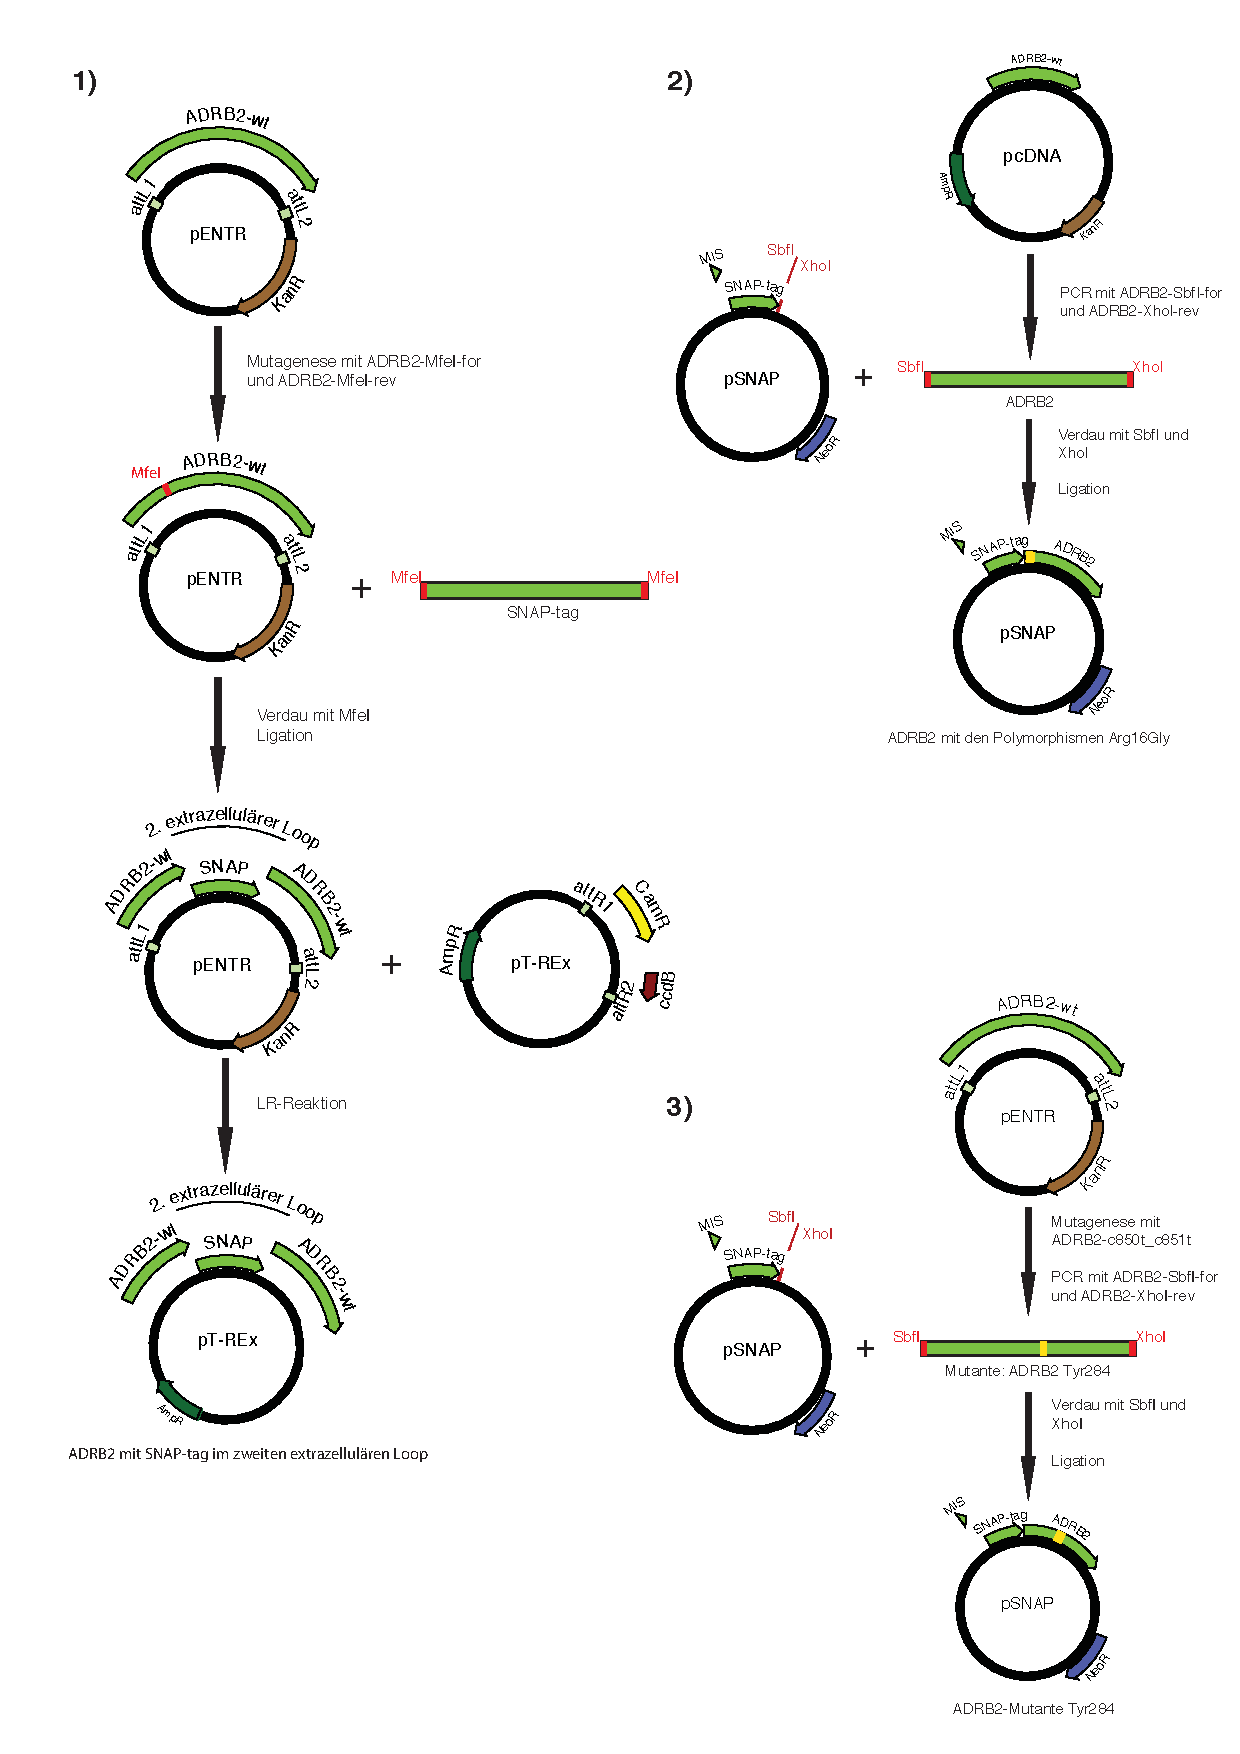
\includegraphics[width=0.97\textwidth]{cloning.pdf}
    \caption{\textbf{Klonierungsstrategien}: \textbf{1)} Generierung eines Expressionsvektors mit dem SNAP-tag im zweiten extrazellulären Loop des \gls{beta2}; \textbf{2)} SNAP-tag am N-Terminus des \gls{beta2}; \textbf{3)} SNAP-tag am N-Terminus der dimerisierungsdefizienten Mutante des \gls{beta2}}
    \label{fig:klonierung}
\end{figure}

\section{Fluoreszenzmikroskopie des \gls{beta2} mit dem SNAP-tag} \label{snapmikro}

Die Charakterisierung der Oligomerisierung des \gls{beta2} zunächst außer Acht gelassen, wurden zuerst Fluoreszenzfärbungen mit SNAP-Substraten durchgeführt. Dabei sollte geprüft werden, ob der mit dem SNAP-tag versehene Rezeptor korrekt in die Zellmembran integriert wird, bzw. noch trivialer, ob die Transfektion mit zufriedenstellender Effizienz gelungen war.

Wie in \ref{klonierung} beschrieben, konnten erfolgreich Vektoren erzeugt werden, die den mit dem SNAP-tag versehenen \gls{beta2} trugen. Diese Plasmide konnten in die HeLa- und HEK293-Zelllinien transient transfiziert werden.

\begin{figure}[htp]
    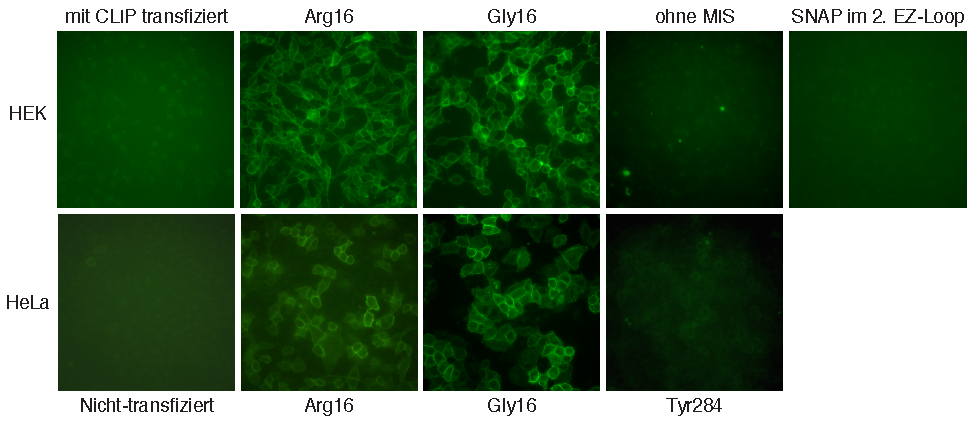
\includegraphics[width=1.0\textwidth]{snap_fluormikro.pdf}
    \caption{\textbf{Fluoreszenzfärbung mit SNAP-Substraten:} transient exprimierende HEK293- und stabile HeLa-Zellen.}
    \label{fig:stainsnap}
\end{figure}

Zunächst wurden direkt nach der Transfektion in HEK293-Zellen mit BG-Alexa-488 SNAP-basierte Fluoreszenzfärbungen durchgeführt. Dabei zeigten sich die in Abbildung \ref{fig:stainsnap} in der mit HEK gekennzeichneten Zeile dargestellten Expressionsmuster: Als Negativkontrolle dienten entweder nicht transfizierte Zellen oder Zellen, die mit dem \gls{beta2} transfiziert worden waren, der den CLIP-tag trug. Für den Arg16Gly-Polymorphismus zeigte sich in beiden Fällen ein deutliches Membranexpressionsmuster mit vernachlässigbarem Hintergrundsignal. Für die Variante des Vektors, der N-terminal vor dem SNAP-tag kein Membraninsertionssignal enthielt, war keine Membranfärbung nachweisbar. Auch die Variante des \gls{beta2}, die den SNAP-tag im zweiten extrazellulären Loop trug, war fluoreszenzmikroskopisch kein Membranexpressionsmuster erkennbar. Die Tyr284-Variante, wurde in HeLa-Zellen transfiziert. Dort war keine Membranfärbung erkennbar.
\\ \\
HEK293-Zellen eigneten sich aufgrund ihrer geringen Adhärenz nicht für die weiteren Versuchsreihen, die allesamt häufiges Waschen benötigten. Somit wurden stabile Zelllinien nur mit den stärker adhärenten HeLa-Zellen generiert. Diese zeigten in der Fluoreszenzmikroskopie eine den HEK293-Zellen vergleichbare Membranexpression. Die Ergebnisse sind in Abbildung \ref{fig:stainsnap} dargestellt. Sowohl bei der Arg16- als auch bei der Gly16-Variante des \gls{beta2} war eine klare lineare Membranfärbung feststellbar.

\section{Oligomerisierung des \gls{beta2} mit SNAP-tag}
Zur Analyse der Oligomerisierung des \gls{beta2} wurde der in der Einleitung beschriebene trFRET-Ansatz verwendet. Dazu wurden zuerst mit trFRET kompatible Fluorophore, die an Substrate des SNAP-tag gekoppelt waren, in unterschiedlichen Versuchsreihen zur Untersuchung der prinzipiellen Oligomerisierung des modifizierten \gls{beta2} eingesetzt. In den in Abschnitt \ref{ligandenfret} vorgestellten Ergebnissen konnten dann fluoreszierende Liganden des unveränderten \gls{beta2} in analogen Versuchsreihen die Oligomerisierung des Rezeptors zeigen.

\subsection{\gls{trfret} mit SNAP-Substraten}
Mit Hilfe der trFRET-Methode konnte die räumliche Interaktion von Molekülen es \gls{beta2} nachgewiesen werden. Dazu wurde in einem ersten Schritt die optimale Konzentration des Donorfluorophors bestimmt. Darauf konnte eine räumliche Interaktion gemessen werden. In einem letzten Schritt wurde gezeigt, dass diese spezifisch war.

\subsubsection{Bestimmung der Sättigungskinetik der SNAP-Substrate}
Zur optimalen Einstellung der Konzentrationen der verwendeten SNAP-Substrate wurden Sättigungsassays durchgeführt. Dazu wurden steigende Konzentrationen des mit dem Donorfluorophor Lumi4 verbundenen SNAP-Substrats (Lumi4-BG) mit Zellen inkubiert, die den SNAP-getaggten \gls{beta2} trugen. Diese Zellen waren zuvor fluoreszenzmikroskopisch auf ihre Expression untersucht worden. Als Negativkontrolle und zur Abschätzung unspezifischer Bindung des SNAP-Substrates dienten nicht-transfizierte Zellen. Über die Messung der Intensität der Fluoreszenz des Donorfluorophores bei 620nm konnte auf die Sättigung der SNAP-tags Rückschluss gezogen werden. Das Ergebnis ist in Abbildung \ref{fig:lumi4binding} dargestellt.
\\ \\
\begin{figure}[htbp]
	\centering
    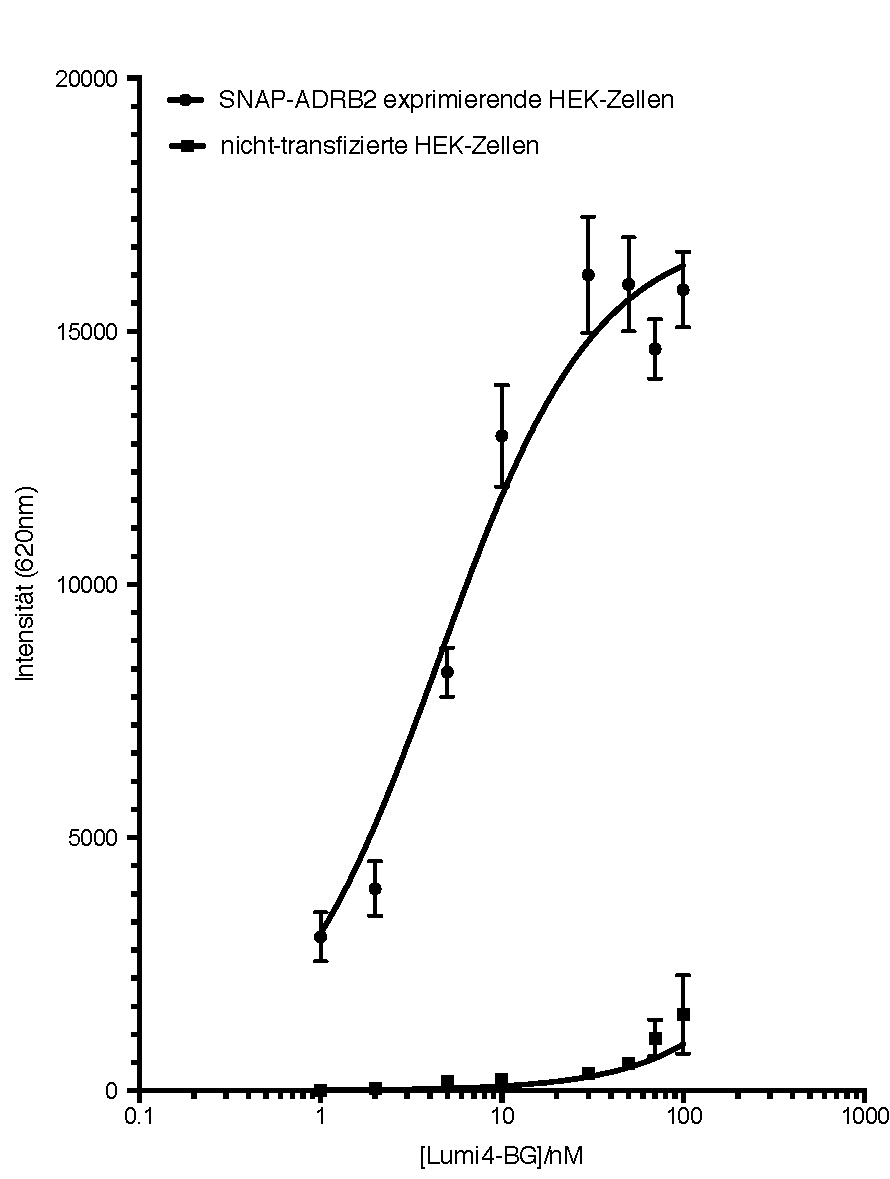
\includegraphics[width=0.6\textwidth]{lumi4binding.pdf}
    \caption{\textbf{Bindungskinetik des Lumi4-Donorfluorophors}}
    \label{fig:lumi4binding}
\end{figure}
Über steigenden Konzentrationen des SNAP-Substrates zeigte sich ein sigmoider Intensitätsverlauf, der bei spezifischer sättigbarer Bindung zu erwarten ist. Die unspezifische Bindung erwies sich als gering. Für die weitere Analyse waren mehrere Bedingungen zu optimieren: Zum einen sollte die Konzentration der SNAP-Substrate gering gehalten werden, um nicht-spezifische Bindung vernachlässigen zu können. Zum anderen war für eine zufriedenstellende signal-to-noise-ratio eine ausreichend hohe Konzentration zu wählen.

Diese Bedingung waren am besten bei der etwa halbmaximal sättigenden Konzentration des SNAP-Substrates gegeben. Für die Analyse der spezifischen Interaktion der SNAP-getaggten Rezeptoren wurde daher die Konzentration des Donor-Substrates auf 10\si{\nano M} festgelegt.

\subsubsection{Räumliche Interaktion des SNAP-getaggten \gls{beta2}}
\begin{figure}[htbp]
	\centering
    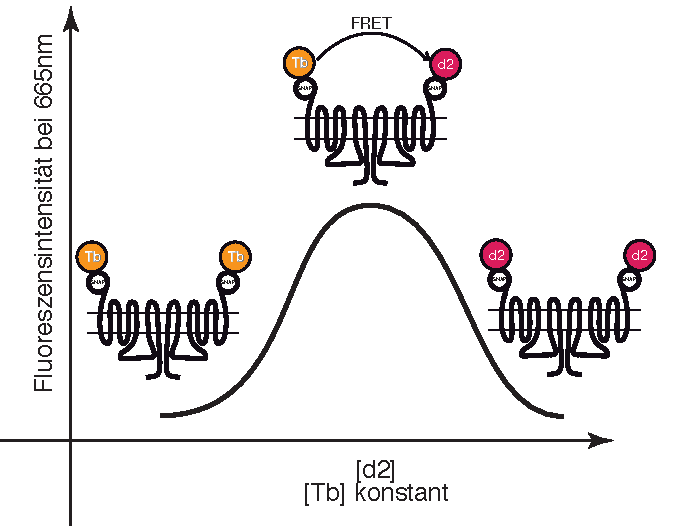
\includegraphics[width=0.5\textwidth]{bell.pdf}
    \caption{\textbf{Maximierung des FRET-Signals}}
    \label{fig:bell}
\end{figure}
    
\subsubsection{Nachweis der spezifischen Interaktion zwischen Rezeptoroligomeren}

\subsection{Einfluss der Stimulation mit Liganden des \gls{beta2} auf seine Oligomerisierung}

\subsection{Einfluss der Glycosylierung auf die Oligomerisierung des \gls{beta2}}

\section{\gls{trfret} mit fluoreszierenden Liganden des \gls{beta2}}
\label{ligandenfret}

